\clearpage
\VerdierPhysicalPageAnchor{0141}%
\begingroup
\small
\setlength{\parskip}{0pt}%
\setlength{\emergencystretch}{1.5em}%
\setlength{\abovedisplayskip}{1pt plus 1pt minus 1pt}%
\setlength{\belowdisplayskip}{1pt plus 1pt minus 1pt}%

\VerdierSemanticAnchor{ch2-2-2-8-stepwise-conditions}
\noindent tel que :

\VerdierSemanticAnchor{ch2-2-2-8-condition-1}
\par\noindent\makebox[1.8em][l]{1)}On ait l'égalité $us_1=tu_1''$ et
$s_1\in S$. Ceci se fait en utilisant SM2).

\VerdierSemanticAnchor{ch2-2-2-8-condition-2}
\par\noindent\makebox[1.8em][l]{2)}On ait les égalités
$mQ(s_1s_2)=Q(f')$, où $f'\colon X_2''\longrightarrow X'$ est un
morphisme de $\mathcal D$, $u_2''=u_1''s_2$ et $s_2\in S$. Ceci se fait
en utilisant le théorème (2.2.2).

\VerdierSemanticAnchor{ch2-2-2-8-condition-3}
\par\noindent\makebox[1.8em][l]{3)}On ait l'égalité
$u'f's_3=gu_2''s_3$, $u''=u_2''s_3$, et $s_3\in S$. En effet, le
diagramme de $\mathcal D$ :

\VerdierSemanticAnchor{ch2-2-2-8-source-square}
\begin{center}
  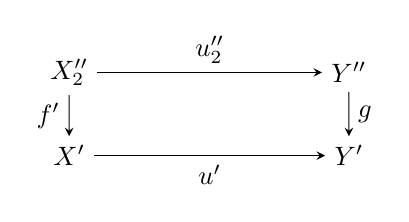
\begin{tikzpicture}[>=stealth,line width=.38pt,x=1.85cm,y=1.10cm,
    scale=.96,transform shape]
    \node (X2pp) at (0,1) {$X_2''$};
    \node (Ypp)  at (2,1) {$Y''$};
    \node (Xp)   at (0,0) {$X'$};
    \node (Yp)   at (2,0) {$Y'$};
    \draw[->] (X2pp) -- node[above] {$u_2''$} (Ypp);
    \draw[->] (X2pp) -- node[left] {$f'$} (Xp);
    \draw[->] (Ypp)  -- node[right] {$g$} (Yp);
    \draw[->] (Xp)   -- node[below] {$u'$} (Yp);
  \end{tikzpicture}
\end{center}

\VerdierSemanticAnchor{ch2-2-2-8-localized-commutativity}
\noindent n'est pas nécessairement commutatif. Mais le diagramme de
$\mathcal D(S^{-1})$ obtenu en appliquant le foncteur $Q$ au diagramme
précédent est commutatif. On a donc
$Q(u'f')=Q(gu_2'')\colon Q(X_2'')\longrightarrow Q(Y')$.

\VerdierSemanticAnchor{ch2-2-2-8-s3-refinement}
Il en résulte, par définition des morphismes de $\mathcal D(S^{-1})$,
qu'il existe un morphisme $s_3\in S\colon X''\longrightarrow X_2''$ tel
que $u'f's_3=gu_2''s_3$.

\VerdierSemanticAnchor{ch2-2-2-8-proof-complete}
Pour achever la démonstration du lemme, il suffit de poser
$f=f's_3$, $s=s_1s_2s_3$.

\VerdierSemanticAnchor{ch2-2-2-9}
\smallskip
\noindent\textbf{2.2.9. Fin de la démonstration du théorème 2.2.6.}
\VerdierSemanticAnchor{ch2-2-2-9-triv-reduction}%
Il reste à démontrer que l'ensemble $T$ possède la propriété TRIV. Nous
savons maintenant que cet ensemble possède les propriétés TRI, TRII et
TRIII. On peut donc utiliser les résultats du numéro 1.2 (1.2.14). En
particulier, il résulte de (1.2.4) que tous les triangles de $T$ contenant
un morphisme donné sont isomorphes. On peut donc, par des réductions
analogues à celles utilisées dans la démonstration de la proposition
(1.3.2), se ramener, pour démontrer la propriété TRIV, à des diagrammes de
$\mathcal D(S^{-1})$ qui sont images par $Q$ de diagrammes analogues de
$\mathcal D$.

\VerdierSemanticAnchor{ch2-2-2-9-reader-details}
La vérification est alors facile. Nous laissons au lecteur le soin d'en
mettre au point les détails.

\VerdierSemanticAnchor{ch2-2-2-10}
\smallskip
\noindent\textbf{2.2.10.}\quad
Soient $\mathcal D$ une catégorie triangulée,
$\mathcal B\subseteq\mathcal D$ une sous-catégorie triangulée pleine et
$S(\mathcal B)$ le système multiplicatif associé à $\mathcal B$
(2.1.15).

\VerdierSemanticAnchor{ch2-2-2-10-quotient-category}
On notera $\mathcal D/\mathcal B$ la catégorie
$\mathcal D(S(\mathcal B)^{-1})$. La catégorie $\mathcal D/\mathcal B$
est appelée la \emph{catégorie quotient de la catégorie $\mathcal D$ par
la catégorie $\mathcal B$}.

\VerdierSemanticAnchor{ch2-2-2-10-quotient-functor}
Le foncteur canonique
$Q\colon\mathcal D\longrightarrow\mathcal D/\mathcal B$ est appelé le
\emph{foncteur de passage au quotient}. Soit
$F\colon\mathcal D\longrightarrow\mathcal D'$ un foncteur exact
(resp. cohomologique) dans une catégorie triangulée (resp. abélienne).

\VerdierSemanticAnchor{ch2-2-2-10-kernel}
On désigne par $\operatorname{Ker}(F)$ et on appelle \emph{noyau de $F$}
la sous-catégorie triangulée strictement pleine saturée définie par les
objets qui sont annulés par $F$ (resp. dont tous les translatés sont
annulés par $F$) ((2.1.16) et (2.1.17)).

\VerdierSemanticAnchor{ch2-2-2-10-p142-boundary}
\endgroup

